 \documentclass{article}
\usepackage{manfnt,amsmath,amsfonts,amssymb}
\usepackage{clrscode3e,latexsym}
\usepackage{graphicx,subfig}
\usepackage[margin=.5in]{geometry}
\usepackage{tikz}
\usepackage{enumitem,booktabs,array}
\usepackage{color}
\title{Graph Algorithms: DAG Shortest Path}\begin{document}\maketitle\newcommand\HR{\rule{.5em}{.4pt}}
\fbox{\begin{minipage}{\linewidth}{\sl Example: Classroom example, directed graph}\end{minipage}}\vspace{1em}


\vspace{1em}


\includegraphics[height=.3\textheight]{dag_shortest_path_00.eps}
\vspace{1em}
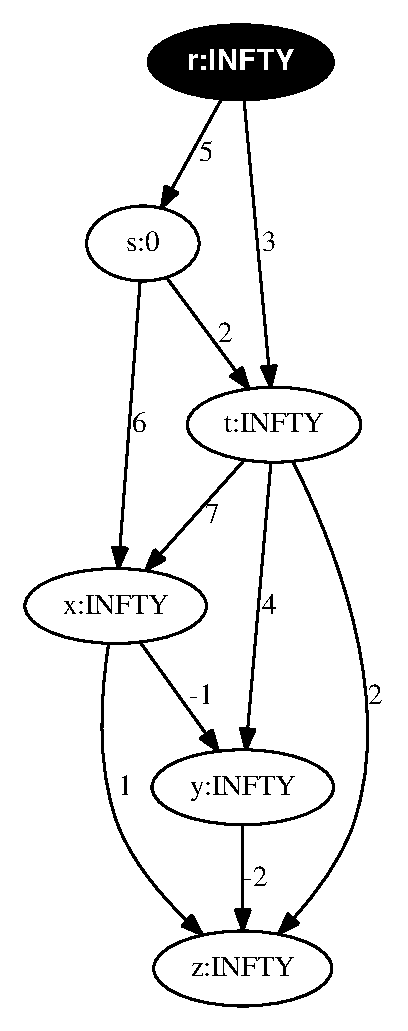
\includegraphics[height=.3\textheight]{dag_shortest_path_01.eps}
\vspace{1em}
\includegraphics[height=.3\textheight]{dag_shortest_path_02.eps}
\vspace{1em}
\includegraphics[height=.3\textheight]{dag_shortest_path_03.eps}
\vspace{1em}
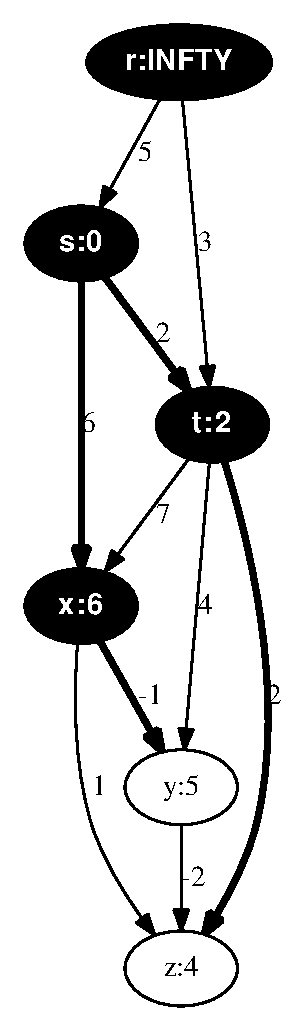
\includegraphics[height=.3\textheight]{dag_shortest_path_04.eps}
\vspace{1em}


\includegraphics[height=.3\textheight]{dag_shortest_path_05.eps}
\vspace{1em}
\includegraphics[height=.3\textheight]{dag_shortest_path_06.eps}
\vspace{1em}
\HR
\begin{minipage}[b][.25\textheight]{0.18181818181818182\linewidth}
The resulting subgraph: 
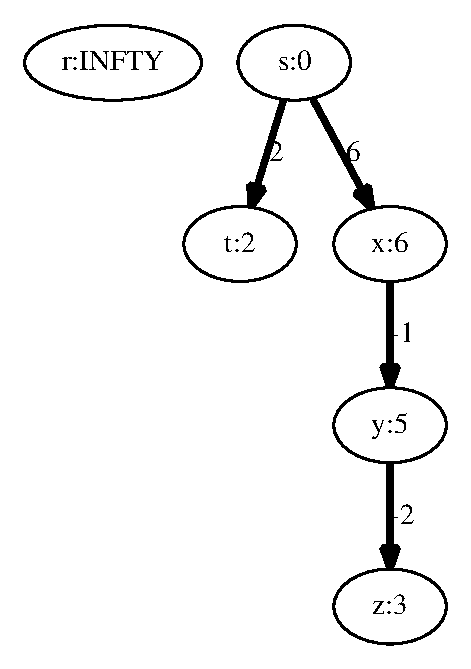
\includegraphics[height=.25\textheight]{dag_shortest_path_07.eps}
\end{minipage}

\end{document}
